\documentclass[12pt]{letter}\usepackage[letterpaper,margin=0.65in]{geometry}\usepackage{textcomp}\usepackage{graphicx}\usepackage[rflt]{floatflt}\pagenumbering{gobble}\begin{document}\begin{floatingfigure}{0.15\textwidth}\raisebox{0pt}[0pt][0pt]{\raisebox{-2.5cm}{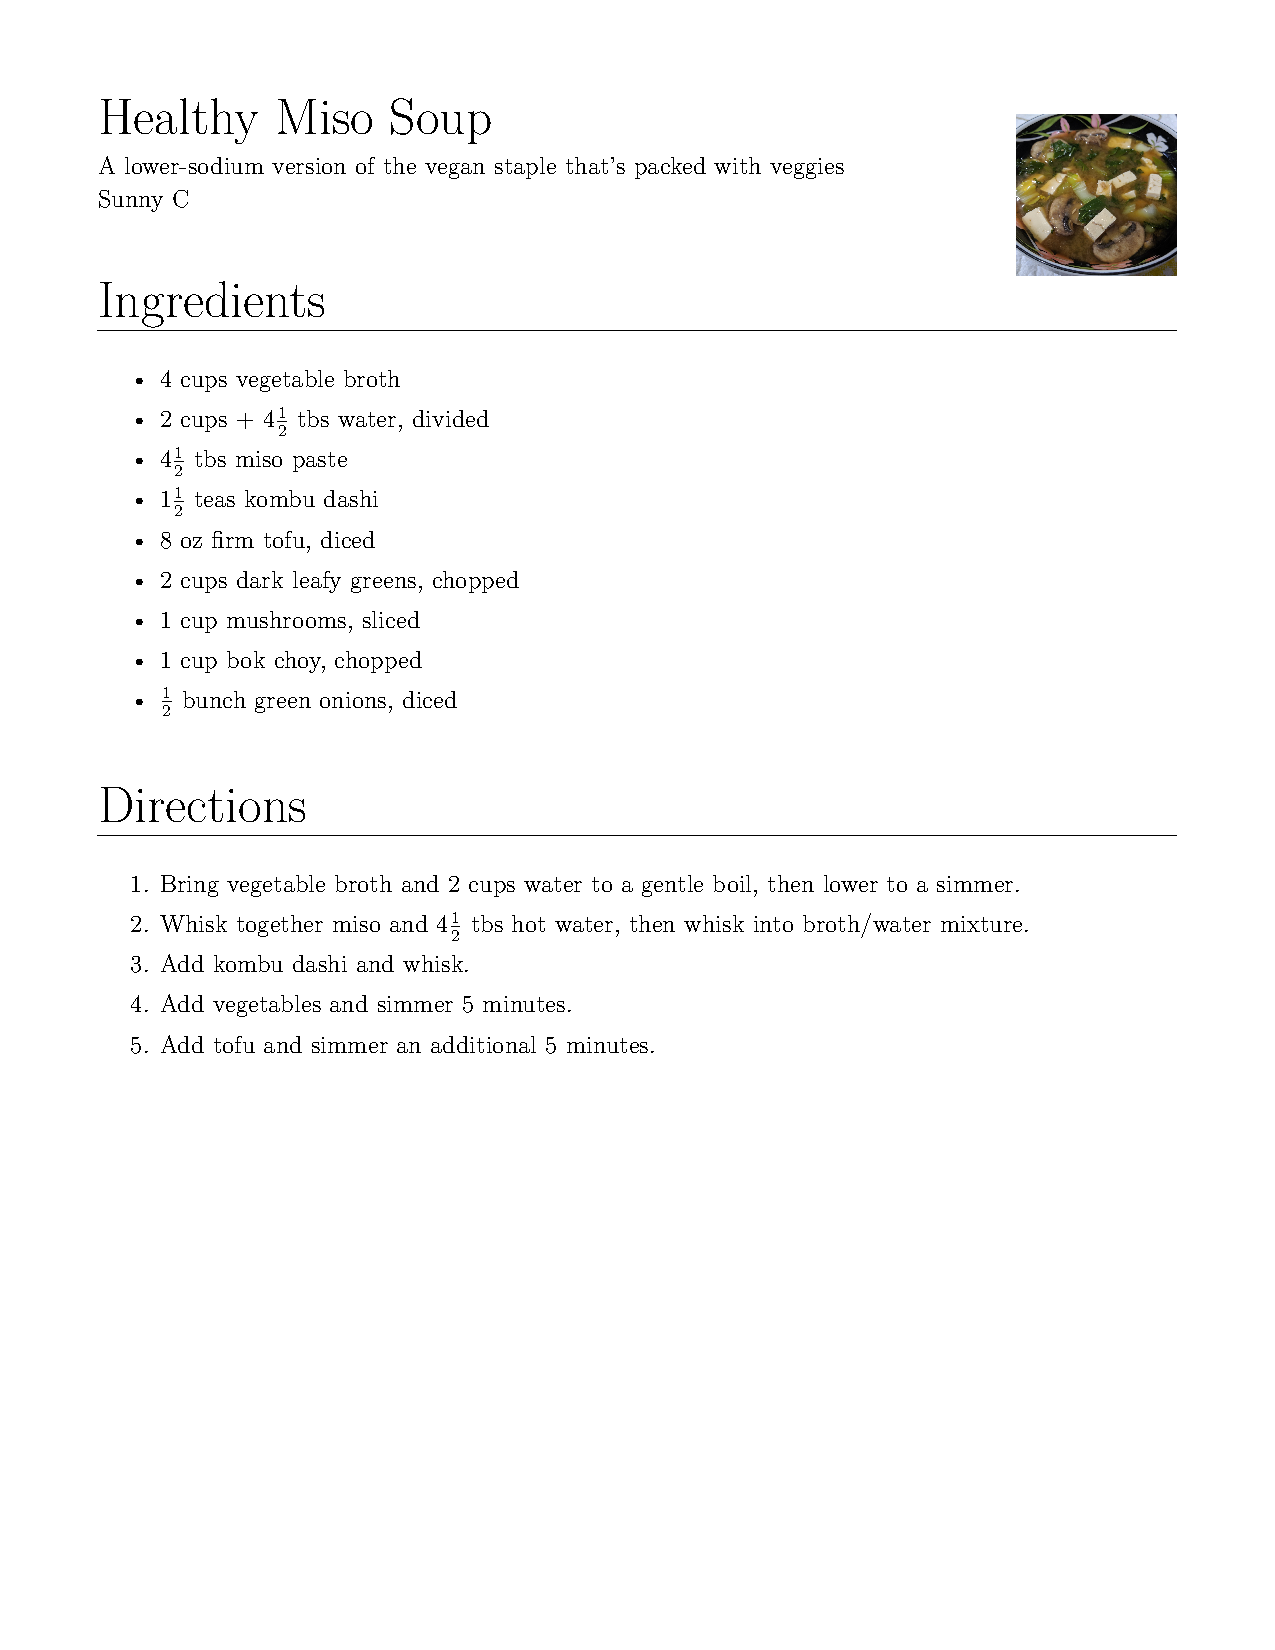
\includegraphics[width=0.15\textwidth]{healthy-miso-soup}}}\end{floatingfigure}\begin{huge}Healthy Miso Soup\end{huge}\newline\vspace{-2.5mm}\newline\renewcommand{\arraystretch}{1.1}\begin{tabular*}{\textwidth}{@{\extracolsep{\fill}}lr}A lower-sodium version of the vegan staple that's packed with veggies\\Sunny C\end{tabular*}\newline\vspace{10mm}\newline\begin{huge}Ingredients\end{huge}\\\rule[2.8mm]{\textwidth}{.1pt}\vspace{-3mm}\begin{itemize}\item 4 cups vegetable broth\item 2 cups + 4$\frac{1}{2}$ tbs water, divided\item 4$\frac{1}{2}$ tbs miso paste\item 1$\frac{1}{2}$ teas kombu dashi\item 8 oz firm tofu, diced\item 2 cups dark leafy greens, chopped\item 1 cup mushrooms, sliced\item 1 cup bok choy, chopped\item $\frac{1}{2}$ bunch green onions, diced\end{itemize}\vspace{7mm}\begin{huge}Directions\end{huge}\\\rule[2.8mm]{\textwidth}{.1pt}\vspace{-3mm}\begin{enumerate}\item Bring vegetable broth and 2 cups water to a gentle boil, then lower to a simmer.\item Whisk together miso and 4$\frac{1}{2}$ tbs hot water, then whisk into broth/water mixture.\item Add kombu dashi and whisk.\item Add vegetables and simmer 5 minutes.\item Add tofu and simmer an additional 5 minutes.\end{enumerate}\end{document}